% This is samplepaper.tex, a sample chapter demonstrating the
% LLNCS macro package for Springer Computer Science proceedings;
% Version 2.21 of 2022/01/12
%
\documentclass[runningheads]{llncs}
%
\usepackage[T1]{fontenc}
% T1 fonts will be used to generate the final print and online PDFs,
% so please use T1 fonts in your manuscript whenever possible.
% Other font encondings may result in incorrect characters.
%
\usepackage{amsmath}
\usepackage{graphicx}
\usepackage{amssymb}
\usepackage{algorithm}
\usepackage{algpseudocode}
\usepackage{tikz}
\usetikzlibrary{arrows.meta, positioning}

\usepackage{fixme}
\usepackage{cancel}
\usepackage{url}
\usepackage{booktabs}
\usetikzlibrary{arrows.meta, positioning}
\fxsetup{status=draft} % <====== add this line
  
\usetikzlibrary{shapes.geometric}
\usepackage{graphicx}
\usepackage{subcaption}
 
\usetikzlibrary{positioning}

\tikzset{
	box/.style={
		draw,
		rectangle,
		rounded corners,
		align=left,
		font=\small,
		inner sep=4pt,
		fill=green!15
	}
}

% Used for displaying a sample figure. If possible, figure files should
% be included in EPS format.
%
% If you use the hyperref package, please uncomment the following two lines
% to display URLs in blue roman font according to Springer's eBook style:
%\usepackage{color}
%\renewcommand\UrlFont{\color{blue}\rmfamily}
%\urlstyle{rm}
%
\begin{document}

	\title{Supplementary file on the paper entitled ``On Solving the Variable Gapped Longest Common Subsequence Problem''}
	
		\author{
		Marko Djukanović\inst{1,2, 6}  \and
		Nikola Balaban\inst{2}   \and
		Christian Blum\inst{3}  \and 
		Aleksandar Kartelj\inst{4}  \and
		Sašo Džeroski\inst{5}  \and
		Žiga Zebec\inst{6}
	}
	%
	\authorrunning{Djukanovic et al.}
	\institute{University of Nova Gorica, Nova Gorica, Slovenia \\ \email{marko.dukanovic@ung.si} \\ \and Faculty of Natural Sciences and Mathematics, University of Banja Luka, Banja Luka, Bosnia and Herzegovina \\
		\email{nikola.balaban@student.pmf.unibl.org}, \email{marko.djukanovic@pmf.unibl.org} \and
		Artificial Intelligence Research Institute (IIIA-CSIC), Barcelona, Spain \\
		\email{christian.blum@iia.csic.es} \and 
		Faculty of Mathematics, University of Belgrade, Belgrade, Serbia \\ \email{kartelj@matf.rs} \\ \and
		Jožef Stefan Institute, Ljubljana, Slovenia \ \\ \email{saso.dzeroski@ijs.si}  \\
		\and
		Institute of Information Sciences (IZUM), Maribor, Slovenia \\
		\email{ziga.zebec@izum.si} \vspace{-0.7cm} \\
	}
	
	
	\maketitle
	\appendix
	\section{ILP model for the fixed $m=2$ VGLCS Problem}\label{app:ilp}
	
	For the case of the VGLCS problem with $m=2$, in this section, we design an
\emph{integer programming model}, representing a methodological approach that differs from
most existing approaches in the literature, which are predominantly based on dynamic
programming (DP). This is a proof-of-concept showing the structural difficulty of this approach and a baseline modeling contribution when solving the fixed version of the tackled problem. Shortly, the purpose of the ILP model is not computational competitiveness but structural modeling and benchmarking. \\

To this end, let:
\begin{itemize}
	\item $M = \{ (i,j) \mid s_1[i] = s_2[j] \}$ denotes the set of all positions where the characters match.
\end{itemize}

For each $(i,j) \in M$, we define a binary variable:
\[
x_{i,j} =
\begin{cases}
	1, & \textrm{if the pair } (i,j) \textrm{ is selected as part of the solution}, \\
	0, & \textrm{otherwise}.
\end{cases}
\]

We introduce additional binary variables $s_{i,j}$ indicating whether the pair $(i,j)$ represents
the \emph{starting position of the subsequence}. \\

\textit{Objective function}. We maximize the number of selected admissible matches:
\[
\max \sum_{(i,j) \in M} x_{i,j}
\]

\textit{Constraints}. The following constraints are imposed:

\begin{enumerate}
	\item \textrm{Predecessors (variable gap).}  
	For each $(i,j) \in M$, we define the set of valid predecessors:
	\[
	\texttt{Pred}(i,j) =
	\{ (i',j') \in M \mid i' < i,\ j' < j,\ i - i' \leq G_{s_1}[i] + 1,\ j - j' \leq G_{s_2}[j] + 1 \}
	\]
	The activation constraint is given by:
	\[
	x_{i,j} \leq \sum_{(i',j') \in \textrm{Pred}(i,j)} x_{i',j'} + s_{i,j}
	\]
	
	\item \textit{Starting position.}  
	At most one starting pair is allowed:
	\[
	\sum_{(i,j) \in M} s_{i,j} \leq 1
	\]
	
	\item \textit{Conflict constraints (character ordering).}  
	Two distinct pairs $(i,j)$ and $(i',j')$ are in conflict if they violate the character order:
	\[
	\textrm{If } (i \leq i' \textrm{ and } j \geq j') \textrm{ or }
	(i \geq i' \textrm{ and } j \leq j'), \textrm{ then:}
	\quad x_{i,j} + x_{i',j'} \leq 1
	\]
	\item \textit{Auxiliary constraints}: $s_{i, j}=1 \Rightarrow x_{i',j'}=0, \forall (i' \leq i-1, j' \leq j-1)$. The constraints are expressed in the following form: 
	$$ \sum_{(i', j') \mid i'\leq i \wedge j'\leq j} x_{i' j'} + s_{i, j} \leq 1, \forall (i, j) \in M$$
\end{enumerate}


\textit{Domains of the variables are given by}
\[
x_{i,j},\ s_{i,j} \in \{0,1\}, \quad \forall (i,j) \in M.
\]

The model is formulated to maximize the number of valid matches forming a common subsequence,
while respecting the ordering of elements and the maximum allowed gaps between consecutive
elements in both sequences.

\section{Pseudocodes of the IMSBS approach}

\begin{algorithm}[H]
	\caption{Rooted Beam Search}
	\label{alg:bs}
	\begin{algorithmic}[1]
		
		\Function{RootedBeamSearch}{$R, S, \{G_i\}_{i=1}^m, \beta, h$}
		\Comment{$r\in R$: root nodes, $S=\{s_1,\dots,s_m\}$, gap constraints $G_i$, beam width $\beta$, heuristic $h$}
		
		\State $s_{\text{best}} \gets \varepsilon$
		\State $B \gets \emptyset$ \Comment{Starting beam}
		%the first extension: TODO
		\ForAll{$v \in R$} \Comment{starting match extensions}
		   \State $B \gets B \cup \{ (p^{L,v}+\textbf{1}, 1) \}$
		\EndFor
		\State $V_{\text{complete}} \gets \emptyset$
		
		\While{$B \neq \emptyset$}
		\State $Children \gets \emptyset$
		
		\ForAll{$v \in B$}
		\If{$v$ is complete}
		\State $V_{\text{complete}} \gets V_{\text{complete}} \cup \{v\}$
		
		\If{$v.l^v > |s_{\text{best}}|$}
		\State $s^v \gets$ Extract partial solution associated with $v$
		\State $s_{\text{best}} \gets s^v$
		\EndIf
		
		\State \textbf{continue}
		\EndIf
		
		\State $C_v \gets$ \Call{Expand}{$v, S, \{G_i\}_{i=1}^m$}
		\State $Children \gets Children \cup C_v$
		\EndFor
		
		\State \Call{Sort}{$Children, h$} \Comment{decreasing order}
		\State $B \gets Children[ \colon \beta]$
		\EndWhile
		
		\State \Return $s_{\text{best}}, V_{\text{complete}}$
		\EndFunction
	\end{algorithmic}
\end{algorithm}


   %pseudocode:
\begin{algorithm}[H]
	\caption{Iterative Multi-source Beam Search (IMSBS) Framework }
	\label{alg:imbs}
	\begin{algorithmic}[1]
		\Require Sequences $S=\{s_1, \dots, s_m\}$; Gap functions $G_{s_i}(\cdot),i=1,\ldots,m$; beam width $\beta>0$; ${sources\_from\_R}>0$; $beam\_iters>0$, heuristics $h, h'$, time limit $t_{{lim}}$
		\Ensure Approximate common subsequence $s_{\textrm{best}}$ which fulfills all gap constraints
		
		\State Initialize $\mathcal{R} \gets \{ (\mathbf{1},0) \}$ \Comment{A set of root nodes}
		
		
		\ForAll{ $a \in \Sigma$} \Comment{Find closest matching positions for each letter}
		\State $\textbf{p}^w_{a} = ({p}^w_{i, a})_{i=1}^m \gets$ minimum position  $p^w_{i, a} \geq 1$ and $s_i[p^w_{i, a}] = a$ (ignore all gap constraints, remove dominated root positions)
		\State $R \gets R \cup \{ (p^w_a, 0)\}$
		\EndFor
		\State $iter \gets 0$
		\State $s_{\textrm{best}} \gets  \varepsilon$
		
		\While{$\mathcal{R} \neq \emptyset \wedge iter < beam\_iters  \wedge t_{lim}$ not exceeded }
		\State Select $\mathcal{L} \subseteq \mathcal{R}$  ${sources\_from\_R}$  and remove them from $\mathcal{R}$ \Comment{ $\mathcal{R}$ prioritized acc. to $h'$}
		%\Comment{$\mathcal{R}$ can be a pr. queue ordered by heuristic $h'$}
		\ForAll{$w \in \mathcal{L}$}
		\State $s_{bwrd}^w, \_ \gets$ 
		\textsc{RootedBeamSearch}(  
		$(\{ (|s_i| - p^w_i)_{i=1}^m, 0\}, S^{rev}, G^{rev}, \beta', h')$
		\Comment{Refine each $w \in \mathcal{L}$}
		\State  $l^w \gets |(s_{bwrd}^w)^{rev}|-1$  \Comment{Update $l^w$, assign the reverse of $s_{bwrd}^w$ without the last letter  to $w$}
		\EndFor
		\State $s_{b}, V_{complete}
		\gets$ 
		\textsc{RootedBeamSearch}($\mathcal{L}, S, G, \beta, h)$ 
		\If{$|s_b| > s_{best}$}
		\State $s_{best} \gets s_b$
		\EndIf
		
		\ForAll{$v \in V_{complete}$}
		
		\ForAll{ $a \in \Sigma$} \Comment{Find closest matching positions for each letter}
		\State $\textbf{p}^w_{a}= ({p}^w_{i, a})_{i=1}^m \gets$ minimum position  $p^w_{i, a} \geq {p}_i^v$ and $s_i[p^w_{i, a}] = a$ (ignore all gap constraints)
		%\If{$|s_{\textrm{best}}| < l^w + \min_{i=1,\dots,m} \{ |s_i| - p^w_i + 1 \}$}    \Comment{cut-off}
		
		\State $\mathcal{R} \gets$ $\mathcal{R} \cup \{r^w = (\textbf{p}^w_a, 0)\}$   (if has not previously been  added) \Comment{Update $\mathcal{R}$}
		% \EndIf
		\EndFor
		\EndFor
		
		\State $iter \gets iter + 1$
		\EndWhile
		
		\State \Return $s_{\textrm{best}}$
	\end{algorithmic}
\end{algorithm}


\begin{figure}[!ht]
  \centering
  \scalebox{0.70}{
	 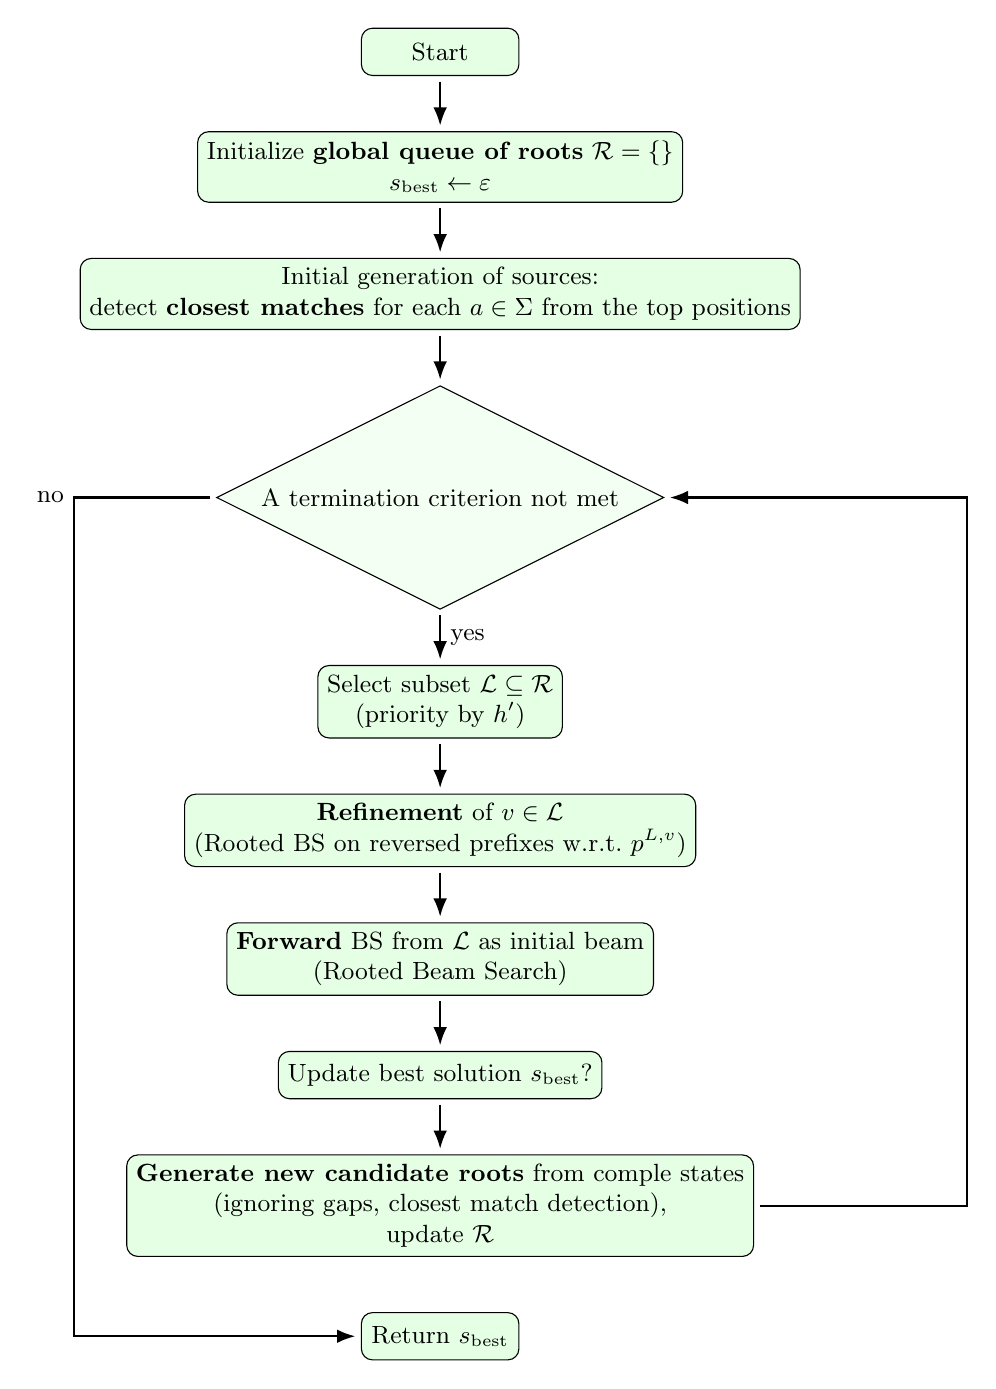
\begin{tikzpicture}[
		node distance=0.7cm and 1.2cm,
		every node/.style={font=\small},
		block/.style={
			rectangle,
			draw,
			rounded corners,
			align=center,
			minimum width=2.0cm,
			minimum height=0.6cm,
			fill=green!10
		},
		decision/.style={
			diamond,
			draw,
			align=center,
			aspect=2,
			fill=green!5
		},
		arrow/.style={
			->,
			thick,
			>=Latex,
			shorten >=2pt,
			shorten <=2pt
		}
		]
		
		% Nodes
		\node[block] (start) {Start};
		
		\node[block, below=of start] (init) {Initialize \textbf{global queue of roots} $\mathcal{R}=\{\}$\\
			$s_{\text{best}} \leftarrow \varepsilon$};
		
		\node[block, below=of init] (expandR) {Initial generation of sources:\\ detect \textbf{closest matches} for each $a \in \Sigma$ from the top positions};
		
		\node[decision, below=of expandR] (while) {A termination criterion not met};
		
		\node[block, below=of while] (selectL) {Select subset $\mathcal{L} \subseteq \mathcal{R}$\\
			(priority by $h'$)};
		
		\node[block, below=of selectL] (backward) {\textbf{Refinement} of $v \in \mathcal{L}$\\
			(Rooted BS on reversed prefixes w.r.t.\ $p^{L,v}$)};
		
		\node[block, below=of backward] (forward) {\textbf{Forward} BS from $\mathcal{L}$ as initial beam\\
			(Rooted Beam Search)};
		
		\node[block, below=of forward] (updateBest) {Update best solution $s_{\text{best}}?$};
		
		\node[block, below=of updateBest] (expandNew) {\textbf{Generate new candidate roots} from comple states\\
			(ignoring gaps, closest match detection), \\ update $\mathcal{R}$};
		
		\node[block, below=of expandNew] (end) {Return $s_{\text{best}}$};
		
		% Arrows (main flow)
		\draw[arrow] (start) -- (init);
		\draw[arrow] (init) -- (expandR);
		\draw[arrow] (expandR) -- (while);
		
		\draw[arrow] (while) -- node[right] {yes} (selectL);
		\draw[arrow] (selectL) -- (backward);
		\draw[arrow] (backward) -- (forward);
		\draw[arrow] (forward) -- (updateBest);
		\draw[arrow] (updateBest) -- (expandNew);
		
		% Explicit loop-back arrow (FIXED)
		\draw[arrow]
		(expandNew.east) -- ++(2.7,0)
		|- (while.east);
		
		% Exit arrow
		\draw[arrow]
		(while.west) -- ++(-1.8,0)
		node[left] {no}
		|- (end.west);		
	\end{tikzpicture}}

  \caption{Simplified workflow of the Iterative Multi-source Beam Search (IMSBS) framework.}
  \label{fig:imsbs_workflow}
\end{figure}


\section{Experimental Evaluation: Tuning \& Numerical Results}

\begin{figure}[H]
	\centering
	\begin{subfigure}[t]{0.48\textwidth}
		\centering
		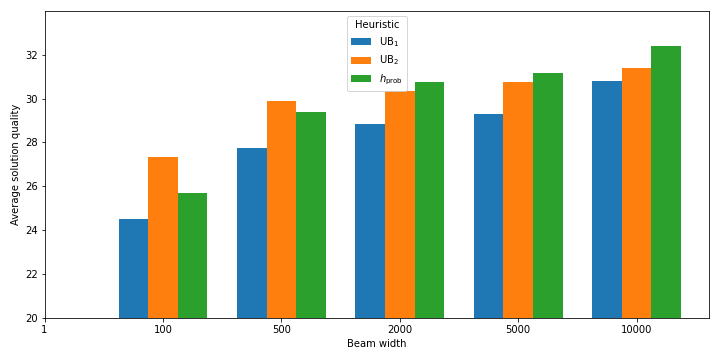
\includegraphics[width=\linewidth, height=120pt]{figures/bs_tuning_quality.png}
		\caption{Avg. quality over all instances of the \textsc{Random} benchmark suite.}
		\label{fig:tune_bs}
	\end{subfigure}
	~
	\begin{subfigure}[t]{0.48\textwidth}
		\centering
		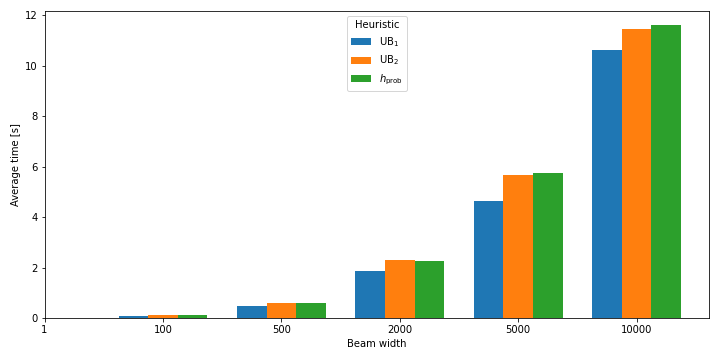
\includegraphics[width=\linewidth, height=120pt]{figures/bs_tuning_time.png}
		\caption{Avg. runtime over all instances of the \textsc{Random} benchmark suite.}
		\label{fig:tune_bs_time}
	\end{subfigure}
	\caption{Beam search tuning results on the \textsc{Random} benchmark suite.}
	\label{fig:bs_tuning}
\end{figure}

\begin{figure}[!h]
	\centering
	\begin{minipage}{0.48\textwidth}
		\centering
		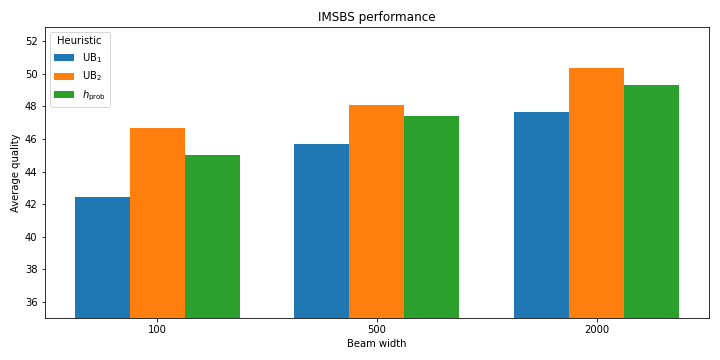
\includegraphics[width=\linewidth]{figures/imsbs_tuning.png}
		\caption*{(a) Avg. solution quality of different IMSBS settings over all instances of the \textsc{Random} benchmark suite.}
		\label{fig:tune_imsbs}
	\end{minipage}
	~
	\begin{minipage}{0.48\textwidth}
		\centering
		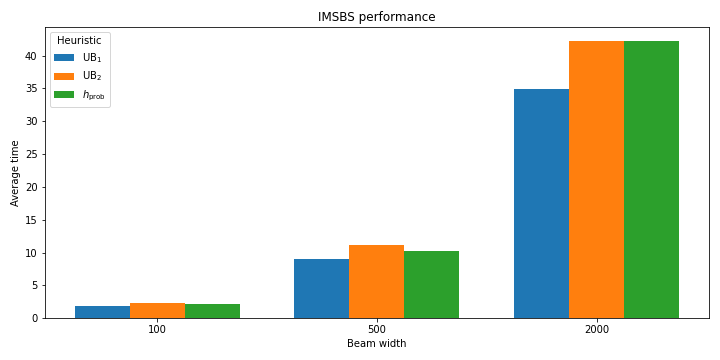
\includegraphics[width=\linewidth]{figures/imsbs_tuning_time.png}
		\caption*{(b) Avg. runtime of different IMSBS settings over all instances of the \textsc{Random} benchmark suite.}
		\label{fig:tune_imsbs_time}
	\end{minipage}
	\caption{IMSBS parameter tuning results on the \textsc{Random} benchmark suite.}
	\label{fig:imsbs_tuning}
\end{figure}

   
     Numerical results for all three heuristic derivatives are shown in Table~\ref{tab:numerical_results_general_m}.   organized as follows. 
     First three columns describe the instance characteristics: the number of sequences ($m$), the sequence length ($n$), and the alphabet size ($|\Sigma|$).  The remaining columns report the performance metrics of three heuristic approaches: \textsc{Bs}, \textsc{Imsbs-greedy}, and \textsc{Imsbs} respectively, each by its own block where two performance indicators are reported: the average objective value ($\overline{obj}$) and the average running time in seconds ($\overline{t}$), computed over 10 instances per group. 
   
\begin{table}[!ht]
	\caption{Numerical results   on the \textsc{Random} benchmark suite. }\label{tab:numerical_results_general_m}
	\centering
	\scalebox{0.70}{
		\begin{tabular}{lll|rr|rr|rr}
			\hline
			\multicolumn{3}{c}{Inst.} & \multicolumn{2}{c}{\textsc{Bs}} & \multicolumn{2}{c}{\textsc{Imsbs-Greedy}} & \multicolumn{2}{c}{\textsc{Imsbs}} \\
			\cmidrule(lrr){1-3} \cmidrule(lr){4-5} \cmidrule(lr){6-7} \cmidrule(lr){8-9} \\ 
			$m$ & $n$ & $|\Sigma|$ & $\overline{obj}$ & $\overline{t}[s]$ & $\overline{obj}$ & $\overline{t}[s]$ & $\overline{obj}$ & $\overline{t}[s]$ \\
			\hline
			\midrule
			2 &       50 &         2 &            33.6 &         0.02 &                     33.1 &                  0.00 &         \textbf{37.7} &      0.06 \\
			2 &       50 &         4 &            30.1 &         0.98 &                     27.7 &                  0.00 &         \textbf{30.1} &      0.16 \\
			2 &      100 &         2 &            48.9 &         2.07 &                     64.5 &                  0.01 &         \textbf{72.8} &      0.94 \\
			2 &      100 &         4 &            \textbf{62.1} &        11.19 &                     56.9 &                  0.01 &         61.6 &      0.91 \\
			2 &      200 &         2 &            99.1 &        18.56 &                     95.5 &                  0.02 &        \textbf{136.4} &      6.21 \\
			2 &      200 &         4 &           120.5 &        38.15 &                    116.1 &                  0.05 &        \textbf{124.9} &      6.58 \\
			2 &      500 &         2 &            65.3 &        23.27 &                    153.6 &                  0.07 &        \textbf{265.7} &    119.75 \\
			2 &      500 &         4 &           214.6 &       163.69 &                    227.7 &                  0.12 &        \textbf{294.4} &     60.49 \\ \hline
			3 &       50 &         2 &            17.5 &         0.03 &                     27.2 &                  0.00 &         \textbf{31.2} &      0.14 \\
			3 &       50 &         4 &            21.7 &         0.18 &                     21.5 &                  0.00 &         \textbf{22.9} &      0.19 \\
			3 &      100 &         2 &            19.7 &         0.06 &                     41.8 &                  0.01 &         \textbf{58.5} &      3.15 \\
			3 &      100 &         4 &            34.1 &         2.35 &                     43.4 &                  0.03 &         \textbf{48.4} &      5.58 \\
			3 &      200 &         2 &            15.2 &         0.16 &                     63.6 &                  0.02 &         \textbf{90.0} &     22.48 \\
			3 &      200 &         4 &            85.3 &        23.45 &                     77.2 &                  0.08 &         \textbf{97.1} &     72.25 \\
			3 &      500 &         2 &            12.6 &         0.10 &                     69.9 &                  0.07 &        \textbf{102.9} &     53.56 \\
			3 &      500 &         4 &            90.7 &        86.35 &                    104.2 &                  0.29 &        \textbf{187.7} &    412.27 \\ \hline
			5 &       50 &         2 &             4.8 &         0.00 &                     14.9 &                  0.00 &         \textbf{20.0} &      0.36 \\
			5 &       50 &         4 &             8.9 &         0.01 &                     13.6 &                  0.06 &         \textbf{15.3} &      0.79 \\
			5 &      100 &         2 &             6.3 &         0.01 &                     17.7 &                  0.01 &         \textbf{22.4} &      0.57 \\
			5 &      100 &         4 &             5.3 &         0.01 &                     \textbf{23.2} &                 10.85 &         22.1 &      1.44 \\
			5 &      200 &         2 &             5.3 &         0.01 &                     21.6 &                  0.03 &         \textbf{26.6} &      1.07 \\
			5 &      200 &         4 &             6.4 &         0.02 &                     \textbf{32.5} &                604.11 &         {25.7} &      2.10 \\
			5 &      500 &         2 &             5.9 &         0.10 &                     25.5 &                  0.14 &         \textbf{27.9} &      3.22 \\
			5 &      500 &         4 &             6.8 &         0.10 &                     \textbf{43.6} &               1341.25 &         26.9 &      3.52 \\ \hline
			10 &       50 &         2 &             1.7 &         0.00 &                      8.8 &                  2.28 &          \textbf{9.1} &      0.47 \\ 
			10 &       50 &         4 &             1.9 &         0.00 &                      \textbf{7.0} &                508.36 &          6.1 &      1.46 \\
			10 &      100 &         2 &             1.1 &         0.00 &                     \textbf{14.0} &               1421.10 &          8.6 &      0.54 \\
			10 &      100 &         4 &             2.2 &         0.01 &                      \textbf{8.9} &               1800.45 &          {6.3} &      1.51 \\
			10 &      200 &         2 &             2.5 &         0.01 &                     \textbf{13.2} &               1710.49 &         10.3 &      0.77 \\
			10 &      200 &         4 &             2.2 &         0.02 &                      \textbf{7.9} &               1800.54 &          6.1 &      1.74 \\
			10 &      500 &         2 &             1.8 &         0.08 &                     \textbf{13.8} &               1611.70 &          {9.5} &      1.53 \\
			10 &      500 &         4 &             1.9 &         0.09 &                      \textbf{8.2} &               1800.46 &          6.1 &      2.37 \\
			\hline \hline
			\textbf{Avg.} &  &  &  32.38 & 10.97 & 46.82 & 394.14 &  \textbf{59.73} & 24.63  \\ \hline \hline
	\end{tabular}}
\end{table}

\section{Numerical results for the $m=2$ case}

  In this section, we compare the results of approaches from the literature that are specialized for the case $m=2$. The competitors are listed below and are described in detail in~\cite{penga2011longest}.

\begin{itemize}
	\item \textsc{Dp}: the basic dynamic programming algorithm;
	\item \textsc{Dp}-1: an advanced dynamic programming approach that uses Incremental Suffix Maximum Queries (ISMQ) with \texttt{Col} and \texttt{All} matrices to accelerate the basic DP algorithm;
	\item \textsc{Dp}-2: an enhanced dynamic programming algorithm that handles ISMQ using a \textit{dequeue} data structure for further speedup. All three DP approaches are from \cite{penga2011longest}. Note that the original paper proposes answering ISMQ using Union-Find operations; however, due to a lack of implementation details, we decided to employ a dequeue-based approach in our implementation.
	\item \textsc{Ilp}: an integer linear programming method proposed in this work (see Appendix~\ref{app:ilp}), motivated by the ILP model for the LCS problem~\cite{blum2016metaheuristics}.
\end{itemize}

Each algorithm was allocated 30 minutes of execution time. The \textsc{Ilp} model was solved using the general-purpose solver \textsc{Cplex} version 22.1.

The results are reported in Table~\ref{tab:results-2d-literature}, which is organized as follows. The first three columns describe the characteristics of the instance groups, over which the results are averaged (10 instances per group). The remaining columns report the performance of the four algorithms: \textsc{Dp}, \textsc{Dp}-1, \textsc{Dp}-2, and \textsc{Ilp}. For each approach, both the average solution quality and the average execution time are provided across the 10 instances.


\begin{table}[H]
	\caption{Results on the \textsc{Random} benchmark set for $m=2$: the exact approaches from the literature.}\label{tab:results-2d-literature}
	\centering
	\scalebox{0.9}{
		\begin{tabular}{lll|lr|rr|rr|rr}
			\hline
			\multicolumn{3}{c}{Inst.} & \multicolumn{2}{c}{\textsc{Dp}}  &
			\multicolumn{2}{c}{\textsc{Dp-1}} & \multicolumn{2}{c}{\textsc{Dp-2}} & 
			\multicolumn{2}{c}{\textsc{Ilp}}  \\
			\cmidrule(lrr){1-3} \cmidrule(lr){4-5}
			\cmidrule(lr){6-7} \cmidrule(lr){8-9}
			\cmidrule(lr){10-11} 	\\ 
			$m$ & $n$ & $|\Sigma|$ & $\overline{obj}$ & $\overline{t}[s]$ & $\overline{obj}$  & $\overline{t}[s]$ &$\overline{obj}$  & $\overline{t}[s]$ & $\overline{obj}$  & $\overline{t}[s]$ \\
			\hline
			2 &   50 &         2 &              38.1 &          0.01 & 38.1 &          \textbf{0.01} &              38.1 &          0.01  & 38.1 & 168.3 \\
			2 &   50 &         4 &              30.3 &          \textbf{0.01} &              30.3 &          0.02 &              30.3 &          0.02 & 30.3  & 28.0 \\ \hline
			2 &  100 &         2 &              77.4 &          0.1 &              77.4 &          \textbf{0.03} &              77.4 &          0.05 & -- & -- \\
			2 &  100 &         4 &              62.3 &          0.07 &              62.3 &         \textbf{0.06} &              62.3 &          0.09 & 0.00 & 1800.0 \\ \hline
			
			2 &  200 &         2 &             156.4 &          0.75 &             156.4 &          \textbf{0.13} &             156.4 &          0.16  & -- & -- \\
			2 &  200 &         4 &             127.2 &          0.59 &             127.2 &          \textbf{0.25} &             127.2 &          0.32  & -- & -- \\ \hline
			
			2 &  500 &         2 &             395.9 &         13.57 &             395.9 &          \textbf{0.84}  &             395.9 &          1.05 & -- & -- \\
			2 &  500 &         4 &             317.2 &         10.18 &             317.2 &          \textbf{1.70} & 317.2 &  2.1 & -- &-- \\    
			\hline \hline
	\end{tabular}}
	
\end{table} 


Based on the numerical results reported in Table~\ref{tab:results-2d-literature}, the following conclusions can be drawn:

\begin{itemize}
	\item All three dynamic programming approaches prove to be highly efficient, successfully solving all 80 problem instances to optimality.
	\item The runtimes required by the DP methods to obtain optimal solutions are relatively short, in most cases remaining below 10 seconds.
	\item The \textsc{ILP} approach is capable of solving only the smallest instances with $n=50$. Its execution times are approximately two orders of magnitude higher than those of the DP approaches. For larger instances, particularly those with $n=200$, the ILP model fails to solve even the initial (root) relaxation.
\end{itemize}

\begin{figure}[htbp]
	\centering
	\begin{minipage}{0.48\textwidth}
		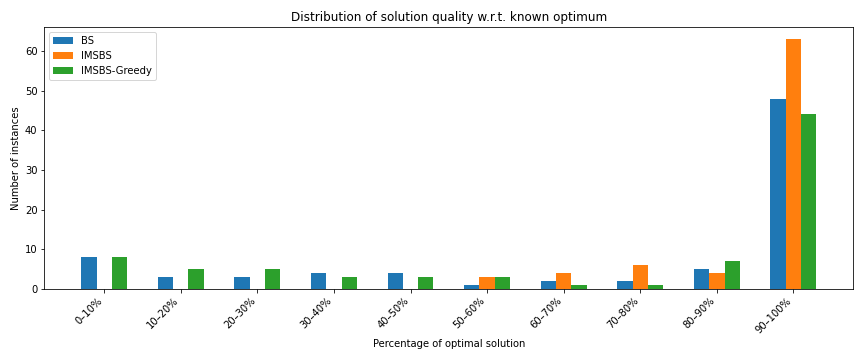
\includegraphics[width=\linewidth,height=120pt]{figures/bs_imsbs_imbs_greedy_vs_dp_quality_distribution.png} 
		\caption*{(a) Percentage distribution of relative solution quality for each heuristic approach with respect to the optimal solutions.} 
	\end{minipage}
	\hfill
	\begin{minipage}{0.48\textwidth}
		\centering
		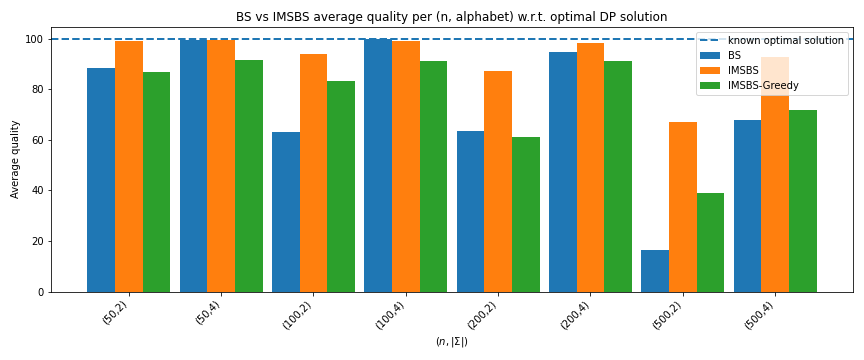
\includegraphics[width=\linewidth,height=120pt]{figures/bs_imsbs_imsbs_greedy_vs_dp_quality.png}
		\caption*{(b) Relative solution quality achieved by the heuristic approaches compared to the optimal solutions.}
	\end{minipage}
	\caption{Number of instances for which \textsc{Bs} and \textsc{Imsbs} achieve a specific relative ratio of the obtained solution quality with respect to the known optimal solutions.}
	\label{fig:optimal-vs-heuristic}
\end{figure}



Concerning the efficiency of \textsc{Bs}, \textsc{Imsbs-Greedy}, and \textsc{Imsbs} on the instances solved optimally by dynamic programming ($m=2$), Figure~\ref{fig:optimal-vs-heuristic} presents the distribution of instances (y-axis) attaining specific ratios of solution quality relative to the known optimal solutions (x-axis).

In particular, \textsc{Imsbs} achieves near-optimal solutions in 63 out of 80 problem instances, whereas the corresponding numbers are significantly lower for the other two heuristic approaches. For instances with $|\Sigma|=4$ (and $m=2$), the difference in solution quality is slightly in favor of \textsc{Imsbs}. However, for instances with a small alphabet ($|\Sigma|=2$), \textsc{Imsbs} clearly outperforms the other two approaches.

Nevertheless, for the group of instances with $n=500$ and $|\Sigma|=2$, there remains room for further improvement. This behavior can be explained by the known weakness of LCS-based heuristics on instances characterized by small alphabet sizes and long sequences; therefore, alternative strategies should be explored, as discussed in the future work section.
\begin{thebibliography}{99}
	
	\bibitem{blum2016metaheuristics}
	C.~Blum and P.~Festa,
	\newblock {\em Metaheuristics for String Problems in Bio-informatics},
	\newblock Vol.~6, John Wiley \& Sons, 2016.
	
	\bibitem{penga2011longest}
	Y.-H.~Penga and C.-B.~Yangb,
	\newblock The Longest Common Subsequence Problem with Variable Gapped Constraints,
	\newblock In {\em Proceedings of the 28th Workshop on Combinatorial Mathematics and Computation Theory, Penghu, Taiwan}, pp.~17--23, 2011.
	
\end{thebibliography}

\end{document}